\documentclass[11pt]{article}
\date{}
\renewcommand\abstractname{\fontsize{14pt}{0}\textbf{Abstract}\selectfont}

\usepackage[left=25mm, right=25mm, top=25mm, bottom=25mm, includehead=false, includefoot=false]{geometry}

\usepackage{graphicx}
\usepackage{url}
\usepackage[round,semicolon]{natbib}  % Citation styles https://www.sharelatex.com/learn/Natbib_citation_styles
\bibliographystyle{humannat}
\renewcommand{\bibsection}{}
\renewcommand{\bibhang}{\setlength{-1px}}


\usepackage{authblk} % For author lists
\renewcommand\Authfont{\fontsize{11}{1}\selectfont}
\renewcommand\Affilfont{\fontsize{9}{1}\selectfont}

\renewcommand*\footnoterule{}

\usepackage[table]{xcolor}
\usepackage[parfill]{parskip} % Line between paragraphs
\usepackage{amsmath}
\pagenumbering{arabic} 

\usepackage{sectsty}
\allsectionsfont{\sffamily}

\usepackage[pdftex]{hyperref} 
\hypersetup{pdfborder={0 0 0} }


% **************  TITLE AND AUTHOR INFORMATION **************

\title{\sffamily\fontsize{16}{0}\textbf{New tools of the trade? The potential and pitfalls of 'Machine Learning' and 'DAGs' to model origin-destination data}}

\author[1]{Robin Lovelace\thanks{}}
\author[2]{Ilan Fridman-Rojas}
\author[3]{Rob Long}
\affil[1]{Institute for Transport Studies, University of Leeds}
\affil[*]{\texttt{Email: R.Lovelace@leeds.ac.uk}}

\usepackage{lmodern}
\usepackage{amssymb,amsmath}
\usepackage{ifxetex,ifluatex}
\usepackage{fixltx2e} % provides \textsubscript
\ifnum 0\ifxetex 1\fi\ifluatex 1\fi=0 % if pdftex
  \usepackage[T1]{fontenc}
  \usepackage[utf8]{inputenc}
\else % if luatex or xelatex
  \ifxetex
    \usepackage{mathspec}
  \else
    \usepackage{fontspec}
  \fi
  \defaultfontfeatures{Ligatures=TeX,Scale=MatchLowercase}
\fi
% use upquote if available, for straight quotes in verbatim environments
\IfFileExists{upquote.sty}{\usepackage{upquote}}{}
% use microtype if available
\IfFileExists{microtype.sty}{%
\usepackage{microtype}
\UseMicrotypeSet[protrusion]{basicmath} % disable protrusion for tt fonts
}{}
\usepackage{hyperref}
\hypersetup{unicode=true,
            pdftitle={Using Machine Learning and Big Data to Model Car Dependency: Progress Report 2 - Machine Learning},
            pdfauthor={Robin Lovelace and Ilan Fridman-Rojas},
            pdfborder={0 0 0},
            breaklinks=true}
\urlstyle{same}  % don't use monospace font for urls
\usepackage{color}
\usepackage{fancyvrb}
\newcommand{\VerbBar}{|}
\newcommand{\VERB}{\Verb[commandchars=\\\{\}]}
\DefineVerbatimEnvironment{Highlighting}{Verbatim}{commandchars=\\\{\}}
% Add ',fontsize=\small' for more characters per line
\usepackage{framed}
\definecolor{shadecolor}{RGB}{248,248,248}
\newenvironment{Shaded}{\begin{snugshade}}{\end{snugshade}}
\newcommand{\KeywordTok}[1]{\textcolor[rgb]{0.13,0.29,0.53}{\textbf{{#1}}}}
\newcommand{\DataTypeTok}[1]{\textcolor[rgb]{0.13,0.29,0.53}{{#1}}}
\newcommand{\DecValTok}[1]{\textcolor[rgb]{0.00,0.00,0.81}{{#1}}}
\newcommand{\BaseNTok}[1]{\textcolor[rgb]{0.00,0.00,0.81}{{#1}}}
\newcommand{\FloatTok}[1]{\textcolor[rgb]{0.00,0.00,0.81}{{#1}}}
\newcommand{\ConstantTok}[1]{\textcolor[rgb]{0.00,0.00,0.00}{{#1}}}
\newcommand{\CharTok}[1]{\textcolor[rgb]{0.31,0.60,0.02}{{#1}}}
\newcommand{\SpecialCharTok}[1]{\textcolor[rgb]{0.00,0.00,0.00}{{#1}}}
\newcommand{\StringTok}[1]{\textcolor[rgb]{0.31,0.60,0.02}{{#1}}}
\newcommand{\VerbatimStringTok}[1]{\textcolor[rgb]{0.31,0.60,0.02}{{#1}}}
\newcommand{\SpecialStringTok}[1]{\textcolor[rgb]{0.31,0.60,0.02}{{#1}}}
\newcommand{\ImportTok}[1]{{#1}}
\newcommand{\CommentTok}[1]{\textcolor[rgb]{0.56,0.35,0.01}{\textit{{#1}}}}
\newcommand{\DocumentationTok}[1]{\textcolor[rgb]{0.56,0.35,0.01}{\textbf{\textit{{#1}}}}}
\newcommand{\AnnotationTok}[1]{\textcolor[rgb]{0.56,0.35,0.01}{\textbf{\textit{{#1}}}}}
\newcommand{\CommentVarTok}[1]{\textcolor[rgb]{0.56,0.35,0.01}{\textbf{\textit{{#1}}}}}
\newcommand{\OtherTok}[1]{\textcolor[rgb]{0.56,0.35,0.01}{{#1}}}
\newcommand{\FunctionTok}[1]{\textcolor[rgb]{0.00,0.00,0.00}{{#1}}}
\newcommand{\VariableTok}[1]{\textcolor[rgb]{0.00,0.00,0.00}{{#1}}}
\newcommand{\ControlFlowTok}[1]{\textcolor[rgb]{0.13,0.29,0.53}{\textbf{{#1}}}}
\newcommand{\OperatorTok}[1]{\textcolor[rgb]{0.81,0.36,0.00}{\textbf{{#1}}}}
\newcommand{\BuiltInTok}[1]{{#1}}
\newcommand{\ExtensionTok}[1]{{#1}}
\newcommand{\PreprocessorTok}[1]{\textcolor[rgb]{0.56,0.35,0.01}{\textit{{#1}}}}
\newcommand{\AttributeTok}[1]{\textcolor[rgb]{0.77,0.63,0.00}{{#1}}}
\newcommand{\RegionMarkerTok}[1]{{#1}}
\newcommand{\InformationTok}[1]{\textcolor[rgb]{0.56,0.35,0.01}{\textbf{\textit{{#1}}}}}
\newcommand{\WarningTok}[1]{\textcolor[rgb]{0.56,0.35,0.01}{\textbf{\textit{{#1}}}}}
\newcommand{\AlertTok}[1]{\textcolor[rgb]{0.94,0.16,0.16}{{#1}}}
\newcommand{\ErrorTok}[1]{\textcolor[rgb]{0.64,0.00,0.00}{\textbf{{#1}}}}
\newcommand{\NormalTok}[1]{{#1}}
\usepackage{longtable,booktabs}
\usepackage{graphicx,grffile}
\makeatletter
\def\maxwidth{\ifdim\Gin@nat@width>\linewidth\linewidth\else\Gin@nat@width\fi}
\def\maxheight{\ifdim\Gin@nat@height>\textheight\textheight\else\Gin@nat@height\fi}
\makeatother
% Scale images if necessary, so that they will not overflow the page
% margins by default, and it is still possible to overwrite the defaults
% using explicit options in \includegraphics[width, height, ...]{}
\setkeys{Gin}{width=\maxwidth,height=\maxheight,keepaspectratio}
\IfFileExists{parskip.sty}{%
\usepackage{parskip}
}{% else
\setlength{\parindent}{0pt}
\setlength{\parskip}{6pt plus 2pt minus 1pt}
}
\setlength{\emergencystretch}{3em}  % prevent overfull lines
\providecommand{\tightlist}{%
  \setlength{\itemsep}{0pt}\setlength{\parskip}{0pt}}
\setcounter{secnumdepth}{5}
% Redefines (sub)paragraphs to behave more like sections
\ifx\paragraph\undefined\else
\let\oldparagraph\paragraph
\renewcommand{\paragraph}[1]{\oldparagraph{#1}\mbox{}}
\fi
\ifx\subparagraph\undefined\else
\let\oldsubparagraph\subparagraph
\renewcommand{\subparagraph}[1]{\oldsubparagraph{#1}\mbox{}}
\fi

%%% Use protect on footnotes to avoid problems with footnotes in titles
\let\rmarkdownfootnote\footnote%
\def\footnote{\protect\rmarkdownfootnote}

%%% Change title format to be more compact
\usepackage{titling}

% Create subtitle command for use in maketitle
\newcommand{\subtitle}[1]{
  \posttitle{
    \begin{center}\large#1\end{center}
    }
}


\begin{document}


\maketitle

% **************  ABSTRACT  **************

\begin{abstract}
\noindent
\setlength{\parindent}{0pt}

This paper explores the potential for emerging methods Machine Learning and Directed Acyclic Graphs (DAGs) to be applied to transport modelling at the origin-destination (OD) level.
OD data is inherently spatial and is complex, due to the multitude of ways of allocating geographic attributes to the OD pairs (e.g. buffers and intersections with geographic representations of OD data generated using straight desire lines, shortest path algorithms or probabilistic routing).
This makes their analysis an interesting geocomputational challenge, seldom tackled by geographers.
The application of Machine Learning and DAG methods, developed in other fields, to this geographical data holds great potential to improve the ability to infer causality in mode split from OD data. However, there are also pitfalls to using these methods which can be black boxes, even if the code is open source, if the analyst does not understand what they are doing with the data.
Based on the work we discuss ways to ensure new methods in the field are used wisely and set-out next steps for our own research.


$ $ \\ {\bf Keywords:} Machine Learning, Causal Inference.

\end{abstract}


\section{Introduction}\label{introduction}

This paper aims to show the potential benefits, and the pitfalls, of
machine learning algorithms in analysing transport data. It results from
a 3 month `T-TRIG' (Transport Technology Research Innovation Grant)
project funded by the UK's Department for Transport (DfT) entitled
``Using Machine Learning and Big Data to Model Car Dependency: an
Exploration Using Origin-Destination Data''.

Despite the applied title, the prime focus was methodological
development: using geocomputation, in the form of new analysis of new
open geographical data, to explore a long-standing policy challenge: how
to reduce car dependency. As highlighted by the DfT, Machine Learning is
relatively new in the transport sector (Hagenauer and Helbich 2017). The
research was therefore exploratory and open-ended in its scope. Having
completed the first Phase of the work (we will have completed the
project in time for the Geocomputation conference), we would like to
comunicate some of the findings from the research.

By demonstrating previously impossible or inaccessible methods we aim to
show how new techniques, combined with new and newly open datasets, can
generate a strong evidence base for transport planning and policy. The
aspiration is that the work will filter into policies, to make them
data-driven, transparent, reproducibible and encouraging of citizen
science and innovation.

\section{Input data}\label{input-data}

For simplicity and maximum accessibility this project uses only datasets
which are open (publicly available). There are three main input dataset
types:

\begin{itemize}
\tightlist
\item
  Origin-destination (OD) commute data from the 2011 Census data.
\item
  Geographically aggregated socio-demographic data from the 2011 Census.
\item
  Geographic variables associated with each OD pair.
\end{itemize}

The Census was used as the primary input dataset because it provides so
many variables relevant to car dependency. To our knowledge, the breadth
of input datasets have never been analysed together in a single project.

The case study region used for this project was \textbf{West Yorkshire}.
This case study was selected due to the wide range of social and
geographical environments linked to car dependency found here: it
includes rural, urban, deprived and privaledged areas.

\subsection{Origin-destination data}\label{origin-destination-data}

The fundamental input dataset was a table reporting the number of people
travelling, by main mode of transport, commuting to work between
Middle-Super Output Areas (MSOAs, average population:
\textasciitilde{}7,500). This is an open dataset
(\href{http://wicid.ukdataservice.ac.uk/}{available online from the
official WICID data portal}) (dataset WU03EW). The file was downloaded
as \texttt{wu03ew\_v2.zip}, an 11.8 MB zipfile which when unzipped
creates the file 109 MB plain text file \texttt{wu03ew\_v2.csv}, read-in
with the following command:

\begin{Shaded}
\begin{Highlighting}[]
\NormalTok{odall =}\StringTok{ }\NormalTok{readr::}\KeywordTok{read_csv}\NormalTok{(}\StringTok{"data/wu03ew_v2.csv"}\NormalTok{)}
\end{Highlighting}
\end{Shaded}

The result is a data frame the first two columns of which contain a the
code for the MSOA of origin and destination, respectively. The
subsequent columns report number of people whose main mode of travel to
work was:

\begin{itemize}
\tightlist
\item
  work at home (no transport used)
\item
  some form of metro
\item
  train
\item
  bus or coach
\item
  taxi
\item
  motorcycle or scooter
\item
  drive a car or van
\item
  passenger in car or van
\item
  bicycle
\item
  walk
\item
  other
\end{itemize}

We grouped together people who drive or are passengers to estimate car
dependency. Further, we filtered out flows with an origin or destination
outside West-Yorkshire, resulting in \textbf{53,807} OD pairs in the
study region. This amount of data is sufficient for machine learning
algorithms to work and extract complex insights, but small enough for
experimentation and fast iteration of methods.

To convert the non-geographical OD dataset into geographic data we used
the function \texttt{od2line()} from the \textbf{stplanr} R package. The
result is straight lines that can be plotted on the map and about which
geographical variables, such as proximity to motorways, can be
extracted.

\begin{figure}
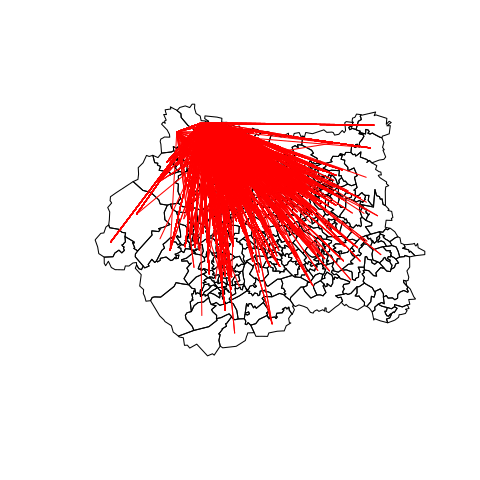
\includegraphics[width=0.49\linewidth]{../figures/flows_500_westyorkshire} 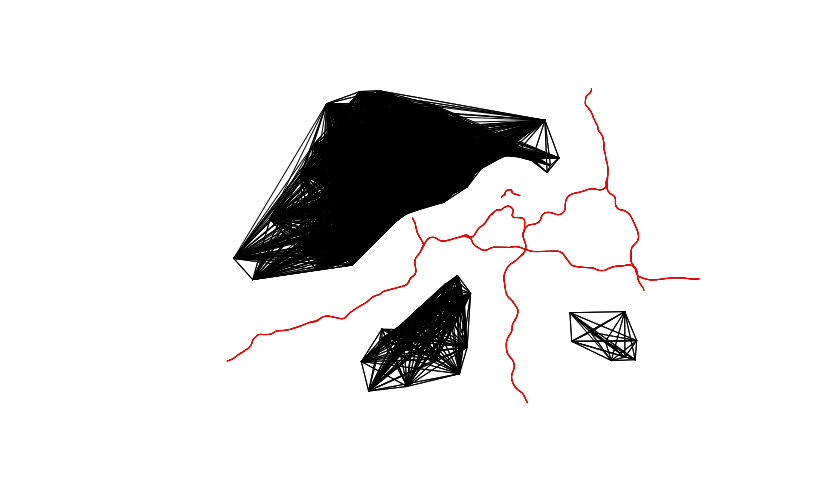
\includegraphics[width=0.49\linewidth]{../figures/dist_motorways} \caption{A sample of work commute flows in the West Yorkshire region (left), and a sample of the result of the code which calculates the distance between motorways (red) and flows (black), in this case discarding all flows within a certain distance of the motorway, as an example.}\label{fig:unnamed-chunk-2}
\end{figure}

We will hereon refer to each home-work (origin-destination) pair and its
corresponding number of commuters, in geographic form, as a \emph{flow}
(see Figure 1).

To this base table there are two ways to further increase the data
included for modelling: the Census provides numerous other demographic
and economic measures and indicators which can be linked to the
commuter's home MSOA
(\href{https://www.nomisweb.co.uk/census/2011/data_finder}{available
here}), and it also provides workplace data which a group of researchers
at the University of Southampton have conveniently created a
classification of (by work type,
\href{http://cowz.geodata.soton.ac.uk/download/}{available online as
well}) which can be linked to the workplace MSOA.

\subsection{Socio-demographic data}\label{socio-demographic-data}

The geodemographic data relevant to each origin (home) MSOA which was
deemed relevant and annexed to the flows data consists of the following
variables: number of people in particular age brackets, number of people
of each gender, car or van availability (including number of homes with
0,1,2,etc. cars), population density, number of economically active and
inactive people, general health (number of people with very good, fair,
etc. general health), number of people per ethnicity group, number of
people by maximum qualification level, and lastly, average number of
rooms, bedrooms and fraction of homes with central heating.

In addition to this we included the workplace zone classification which
assigns each destination MSOA (workplace) to one of 7 groups (Table 1).

\begin{longtable}[]{@{}lr@{}}
\caption{The classification of workplace zones.}\tabularnewline
\toprule
Workplace zone classification & Code\tabularnewline
\midrule
\endfirsthead
\toprule
Workplace zone classification & Code\tabularnewline
\midrule
\endhead
Retail & 1\tabularnewline
Top jobs & 2\tabularnewline
Metro suburbs & 3\tabularnewline
Suburban services & 4\tabularnewline
Manufacturing and distribution & 5\tabularnewline
Rural & 6\tabularnewline
Servants of society & 7\tabularnewline
\bottomrule
\end{longtable}

\subsection{Spatial data}\label{spatial-data}

In addition to this Census data we gathered and computed spatial data as
well. We have obtained the location of motorways through the
\href{https://osmdatar.github.io/osmdata/articles/osmdata.html}{OSM
API}, and the positions of train stations, coach stations, and bus stops
from the \href{http://naptan.app.dft.gov.uk/datarequest/help}{NAPTAN
dataset}. This allowed us to calculate geographical distances between
flow lines and motorways, train stations, coach stations, and bus stops.
This proximity and accessibility data is arguably vital to best
understand and model car usage propensity, and has for the first time
become readily available via the OSM platform, and analysis of the type
we aim to do next should be cutting-edge data analysis.

\newpage

\subsection{Overview of input data}\label{overview-of-input-data}

A sample of the first 20 variables used in the input dataset for the
machine learning algorithms is provided in Table 2 (the full list can be
seen in a code repository that will accompany this paper).

\begin{longtable}[]{@{}ll@{}}
\caption{The first 20 variables in the full dataset.}\tabularnewline
\toprule
Variable & Description\tabularnewline
\midrule
\endfirsthead
\toprule
Variable & Description\tabularnewline
\midrule
\endhead
homeMSOA & MSOA code for origin (place of residence)\tabularnewline
workMSOA & MSOA code for destination (place of work)\tabularnewline
workhome & Fraction of people who work from home (don't
commute)\tabularnewline
metro & Fraction of people who use the metro, tram or light train to
commute\tabularnewline
train & Fraction of people who use the train\tabularnewline
bus & Fraction of people who use the bus\tabularnewline
taxi & Fraction of people who use a taxi\tabularnewline
motorcycle & Fraction of people who use a motorcycle, scooter or
moped\tabularnewline
car & Fraction of people who use a car or are passengers in a car or
van\tabularnewline
cycle & Fraction of people who cycle\tabularnewline
walk & Fraction of people who walk\tabularnewline
othertransp & Fraction of people who use a form of transport not listed
above\tabularnewline
npeople & Total number of people resident in the homeMSOA\tabularnewline
16-24 & Fraction of people in the age range 16-24\tabularnewline
25-34 & Fraction of people in the age range 25-34\tabularnewline
35-49 & Fraction of people in the age range 35-49\tabularnewline
50-54 & Fraction of people in the age range 50-54\tabularnewline
65-74 & Fraction of people in the age range 65-74\tabularnewline
75 & Fraction of people of age 75+\tabularnewline
female & Fraction of people who are female\tabularnewline
\bottomrule
\end{longtable}

\section{Machine Learning}\label{machine-learning}

The first step in this process is that of model selection by
cross-validation, and it is this procedure which we will now describe.
The first step of model selection is to choose the metric of interest,
based on which we will select the best-performing model. Given that this
is a regression problem there are multiple possible metrics: mean
squared error (MSE), mean absolute error, coefficient of determination
(\(R^2\)), etc. From the point of view of policy decision-making, which
is our ultimate goal, there is no clear choice of best-suited metric. We
have chosen the coefficient of determination as it seems to be the
metric of interest for our Data Science contact at the Department for
Transport, but it must be noted that this metric is ill-suited for the
mostly non-linear\footnote{For clarity, we are referring to
  non-linearity in the regression parameters, models non-linear in the
  covariates (e.g.~the Elastic Net model we use) are still linear by
  this definition.} regression models we consider (see for example
(Spiess and Neumeyer 2010)).

Having chosen the metric of interest, we proceed to shuffle and split
the data in preparation for cross-validation. Flows are unordered data
and therefore can be shuffled uniformly with no problem. We shuffle the
flows in the West Yorkshire dataset, and then split off half of the data
for model selection and validation, the other half is left for final
model testing to estimate the generalisation error (or parts of it may
used for further model selection, e.g.~parameter tuning, if needed).

We then perform 10-fold cross-validation on the validation half of the
dataset. At this point we do not perform any hyperparameter tuning and
use the default parameters set in scikit-learn's implementation
(Pedregosa et al. 2011) of these algorithms\footnote{Grid search or
  random search hyperparameter tuning by cross-validation could be
  carried out at a later date on a separate dataset for a subset of the
  selected models to extract further gains in predictive performance.}.
The regression models considered and the result of the model selection
are shown in the table below.

\begin{longtable}[]{@{}lr@{}}
\caption{10-fold cross-validation \(R^2\) scores of the the regression
models considered. The \texttt{MEAN\ MODEL} is a model which always
predicts the mean of the response variable, and is included as a
reference point and benchmark. The RANSAC and Stochastic Gradient
Descent (SGD) regressors have clearly not converged but we will not
attempt to tune them for now.}\tabularnewline
\toprule
Model & \(R^2\)\tabularnewline
\midrule
\endfirsthead
\toprule
Model & \(R^2\)\tabularnewline
\midrule
\endhead
MLP & 9.548066e-01\tabularnewline
XGB & 9.522178e-01\tabularnewline
RandomForest & 9.411053e-01\tabularnewline
ExtraTrees & 9.366043e-01\tabularnewline
ElasticNetCV & 9.268778e-01\tabularnewline
PassiveAggressive & 8.870397e-01\tabularnewline
DecisionTrees & 8.736974e-01\tabularnewline
TheilSen & 8.561763e-01\tabularnewline
KNeighbors & 8.427571e-01\tabularnewline
RANSAC & 7.766147e-01\tabularnewline
--MEAN MODEL-- & 0.000000e+00\tabularnewline
Dummy & -3.752000e-04\tabularnewline
SGD & -1.211319e+23\tabularnewline
\bottomrule
\end{longtable}

Without engaging in extensive hyperparameter tuning on a separate
dataset, we see that the Multi-Layer Perceptron and the XGBoost
regressor (Chen and Guestrin 2016) top the list with
\(R^2 \approx 0.95\). The difference between the top-performing models
is likely not significant, therefore on theoretical grounds we will
choose the XGBoost regressor as our tentative final model, as boosting
is known to be less likely to overfit (Schapire 1999), and therefore is
likely to generalise best to new datasets. We will therefore select it
as a tentative final model and now proceed to perform some model
validation to ensure its predictions are sensible.

\section{Model validation}\label{model-validation}

For a regression task such as the one at hand, the model validation
checks which can be performed are perhaps less intuitive than the tests
available for classification tests. However some basic plots of the
model's predictions and checks of the model's residuals and the
correlation of the model's predictions with observed values can and
should be carried out.

The figure below shows the residuals of the XGBoost regressor on a
validation dataset, showing no obvious trend or asymmetry which would be
indicative of a poorly-fit model.

\begin{figure}

{\centering 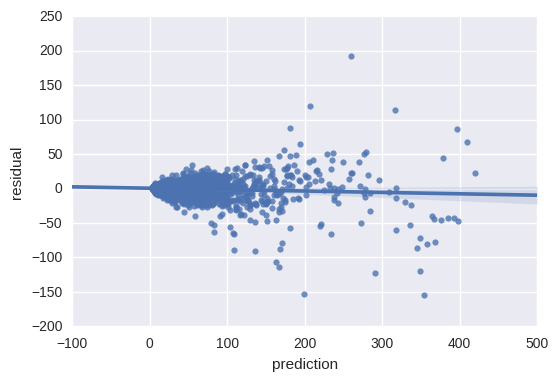
\includegraphics[width=0.49\linewidth]{../figures/xgb_residuals} 

}

\caption{The residuals of the XGBoost regressor on a validation dataset.}\label{fig:unnamed-chunk-3}
\end{figure}

We can further inspect the distribution and correlation of the predicted
and observed values, as well as a histogram of their distribution.

\begin{figure}

{\centering 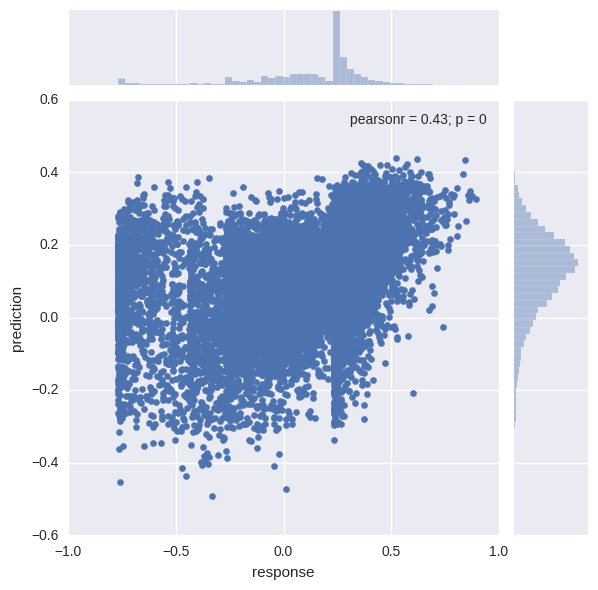
\includegraphics[width=0.49\linewidth]{../figures/xgb_pred_obs_correlation} 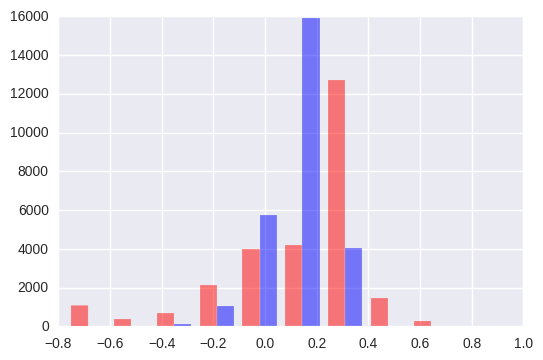
\includegraphics[width=0.49\linewidth]{../figures/xgb_hist} 

}

\caption{The distribution and correlation of predictions and observed values.}\label{fig:unnamed-chunk-4}
\end{figure}

\section{Next steps}\label{next-steps}

There is one noteworthy caveat which applies to all studies using
Machine Learning (and more generally regression on observational data
without Randomised Controlled Trials) to inform decision making: both
Machine Learning approaches and standard regression approaches when
carried out appropriate can identify correlations, but evidence for
these correlations is tentative and correlations by themselves, without
evidence of a causal link, are not a sound basis for decision-making or
interventions.

The patterns found are therefore a very solid first step in finding
potential causal links which could inform decision-making and policy
interventions, but they must be informed by causal modelling. To this
end, in the next stage we will explore introducing causal information
into the machine learning modelling, as well as using standard causal
analysis via the use of Directed Acyclic Graphs (DAGs) to tease out
which correlations may or may not be causal.

The results so far should thus be taken as tentative as they are in the
process of being tested further to guarantee as much as possible their
validity and potential for informed, data-driven decision making.

\section*{References}\label{references}
\addcontentsline{toc}{section}{References}

\hypertarget{refs}{}
\hypertarget{ref-Chen:2016:XST:2939672.2939785}{}
Chen, Tianqi, and Carlos Guestrin. 2016. ``XGBoost: A Scalable Tree
Boosting System.'' In \emph{Proceedings of the 22Nd Acm Sigkdd
International Conference on Knowledge Discovery and Data Mining},
785--94. KDD '16. New York, NY, USA: ACM.
doi:\href{https://doi.org/10.1145/2939672.2939785}{10.1145/2939672.2939785}.

\hypertarget{ref-hagenauer_comparative_2017}{}
Hagenauer, Julian, and Marco Helbich. 2017. ``A Comparative Study of
Machine Learning Classifiers for Modeling Travel Mode Choice.''
\emph{Expert Systems with Applications} 78 (July): 273--82.
doi:\href{https://doi.org/10.1016/j.eswa.2017.01.057}{10.1016/j.eswa.2017.01.057}.

\hypertarget{ref-kursa2010boruta}{}
Kursa, Miron B, Aleksander Jankowski, and Witold R Rudnicki. 2010.
``Boruta--a System for Feature Selection.'' \emph{Fundamenta
Informaticae} 101 (4). IOS Press: 271--85.

\hypertarget{ref-scikit-learn}{}
Pedregosa, F., G. Varoquaux, A. Gramfort, V. Michel, B. Thirion, O.
Grisel, M. Blondel, et al. 2011. ``Scikit-Learn: Machine Learning in
Python.'' \emph{Journal of Machine Learning Research} 12: 2825--30.

\hypertarget{ref-2013arXiv1312.6120S}{}
Saxe, A. M., J. L. McClelland, and S. Ganguli. 2013. ``Exact solutions
to the nonlinear dynamics of learning in deep linear neural networks.''
\emph{ArXiv E-Prints}, December.

\hypertarget{ref-schapire1999brief}{}
Schapire, Robert E. 1999. ``A Brief Introduction to Boosting.'' In
\emph{Ijcai}, 99:1401--6.

\hypertarget{ref-spiess2010evaluation}{}
Spiess, Andrej-Nikolai, and Natalie Neumeyer. 2010. ``An Evaluation of
R2 as an Inadequate Measure for Nonlinear Models in Pharmacological and
Biochemical Research: A Monte Carlo Approach.'' \emph{BMC Pharmacology}
10 (1). Springer: 6.

\hypertarget{ref-srivastava2014dropout}{}
Srivastava, Nitish, Geoffrey E Hinton, Alex Krizhevsky, Ilya Sutskever,
and Ruslan Salakhutdinov. 2014. ``Dropout: A Simple Way to Prevent
Neural Networks from Overfitting.'' \emph{Journal of Machine Learning
Research} 15 (1): 1929--58.

\hypertarget{ref-2016arXiv160502688T}{}
The Theano Development Team, R. Al-Rfou, G. Alain, A. Almahairi, C.
Angermueller, D. Bahdanau, N. Ballas, et al. 2016. ``Theano: A Python
framework for fast computation of mathematical expressions.''
\emph{ArXiv E-Prints}, May.

\hypertarget{ref-vincent2010stacked}{}
Vincent, Pascal, Hugo Larochelle, Isabelle Lajoie, Yoshua Bengio, and
Pierre-Antoine Manzagol. 2010. ``Stacked Denoising Autoencoders:
Learning Useful Representations in a Deep Network with a Local Denoising
Criterion.'' \emph{Journal of Machine Learning Research} 11 (Dec):
3371--3408.


\end{document}
